\subsection{问题二分析}
问题二旨在将问题一得出的司机决策模型,运用到国内某一城市的机场和出租车数据上作为实证分析,并讨论模型的合理性,得出各解释变量对司机选择载客回城的概率$P$的数量关系(正/负相关及具体数值关系)。

本文选择深圳宝安国际机场及出租车数据为例,对问题一中提出的模型做检测。

% \ref{eq:linmodel}

\subsection{解释变量信息汇总}
\subsubsection{深圳出租车计价规则}
\begin{enumerate}[label=\chinese*、]
    \item ``红色''出租小汽车运价项目和标准
        \begin{enumerate}[label=(\chinese*)]
            \item 起步价:首2公里11.00元;
            \item 里程价:超过2公里部分,每公里2.40元;
            \item 返空费:每天的6时23时,超过25公里部分,每公里按上述里程价的30\%加收返空费:
            \item 夜间附加费:夜间起步价16元,每天的23时至次日凌晨6时,按上述起步价和里程价的20\%加收夜间附加费;
            \item 候时费:每分钟0.80元;
            \item 大件行李费:体积超过0.2立方米、重量超过20公斤的大件行李,每件0.50元。
        \end{enumerate}

    \item ``绿色''出租小汽车运价项目和标准
        \begin{enumerate}[label=(\chinese*)]
            \item 起步价:首1.5公里6.00元;
            \item 里程价:超过1.5公里部分,每公里2.40元;
            \item 返空费:每日6时23时,超过15公里部分,每公里按上述里程价的30\%加收返空费;
            \item 夜间附加费:每天的23时至次日凌晨6时,按上述起步价和里程价的20\%加收夜间附加费;
            \item 候时费:每分钟0.50元;
            \item 大件行李费:体积超过0.2立方米、重量超过20公斤的大件行李,每件0.50元。
        \end{enumerate}
\end{enumerate}

因``绿色''清洁能源汽车逐渐普及,故本文采用``绿色''出租车计价规则。


\subsubsection{深圳气候概况二元变量——$weather$}
下表~\ref{tab:weather_report}统计了2016-2018年深圳市极端天气日数,以此作为计算二元变量$weather$取不同状态数时的概率。

\begin{table}
    \centering
    \resizebox{\textwidth}{!}{%
        \begin{tabular}{ccccc}
            \hline
            要素 & 2018年(天) & 2017(天) & 2016年(天) & 累年平均值(天) \\ \hline
            \rowcolor[HTML]{EFEFEF}
            高温日数 & 2 & 7 & 5 & 4.3 \\
            低温日数 & 1 & 0 & 2 & 1.1 \\
            \rowcolor[HTML]{EFEFEF}
            大风日数 & 3 & 2 & 2 & 4.4 \\
            暴雨日数 & 8 & 11 & 11 & 9.2 \\
            \rowcolor[HTML]{EFEFEF}
            雾日数 & 0 & 0 & 3 & 3.3 \\
            霾日数 & 20 & 22 & 27 & 72 \\ \hline
        \end{tabular}%
    }
    \caption{2016--2018年深圳国家基本气象站天气日数}\label{tab:weather_report}
\end{table}

由此得
\[weather = 
    \begin{cases}
        1, & p = 34/365 = 0.093 \\
        0, & p = 1 - 0.093 = 0.907
    \end{cases}.
\]

\begin{figure}
    \centering
    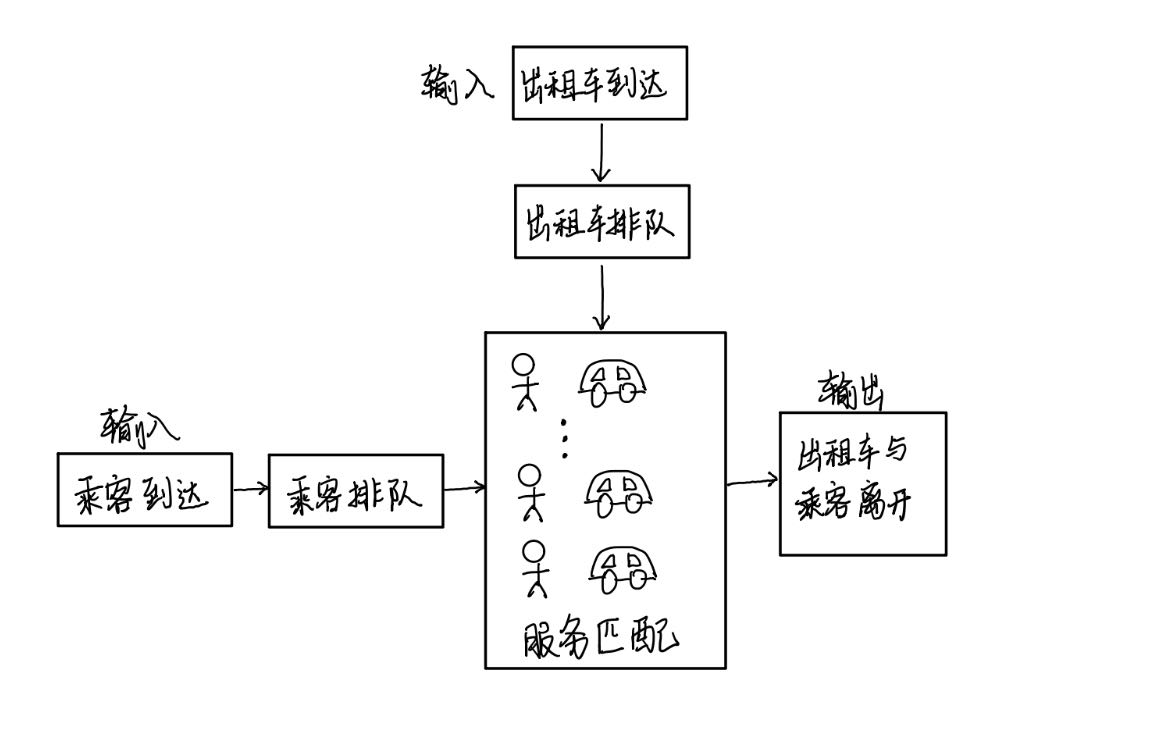
\includegraphics[width=.6\textwidth]{service.jpg}
    \caption{服务布局系统简图}\label{fig:service}
\end{figure}

\subsubsection{司机等待时长$t_d$}
假设司机等待时长服从泊松分布,即$t_{d}\~Poisson(30)$,单位为分钟。

对于排队或说等待问题来说,需考虑的因素是排队长度$L$和顾客等待时间$W$,无论是从系统的角度还是从顾客的角度来看,两者均是越小越好。对服务布局系统进行了研究,如图~\ref{fig:service}。其中队列长$L_q$是指系统中正处于排队等待的平均旅客数,队长$L_S$则是指队列长$L_q$与正在接受服务的顾客数之和。等待时间$W_q$则是指顾客从进入系统开始到开始接受服务的平均时间,逗留时间$W_s$是指从顾客进入系统到接受完服务离开系统的平均时间。

用系统中乘客排队的队长$L_s$及其逗留时间$W_s$对系统进行分析,得:
\begin{equation}\label{eq:排队系统乘客队长-1}
    L_s = L_q + C_\rho = \frac{1}{C!}\frac{(C\rho)^C\rho}{(1-\rho)^2}P_0 + \frac{\lambda}{\mu},
\end{equation}

\subsubsection{行李重量$m$}
大部分民航公司的免费托运行李额为20kg,而实际旅程中乘客携带行李重量层次不一,且尚无直接渠道得到旅客行李托运信息,因此本文认为$m$是不易观测变量,建议使用其他代理变量加入到回归式中。

$m$对民航公司是显式直接以观测变量,本文建议在实际问题解决中考虑该变量对总概率$P$的影响。

% \subsection{到达旅客中意愿乘出租车的人数$N_p$}

% \subsection{模型合理性}
% \subsection{因变量与解释变量数量关系}
%    着重看正/负相关
